\chapter{Caratteristiche pluviometriche dell’area di studio}\label{cap:pluviometriche}
\section{Curve di possibilità pluviometrica}
Dopo che si è eseguito un primo inquadramento della zona si procede con le elaborazioni dei dati dei massimi annuali degli scrosci e delle precipitazioni orarie ricavate dalla stazione pluviometrica di Laste a Trento.
Attraverso queste elaborazioni, svolte attraverso il metodo di BOOOOO(momenti o minimi quadrati o massima verosimiglianza) si pone l'obiettivo di determinare le curve di possibilità pluviometrica (Fig.2) e i propri parametri (Tab.1 (a[mm/h alla n];n)) con diversi tempi di ritorno ($T_r$). 
Per la relazione si considera un tempo di ritorno pari a \si{25} anni. Nella Fig.2, dove si confrontano le CPP degli scrosci e delle precipitazioni orarie, si evince che si ottiene una maggiore altezza di precipitazione, dovuta agli scrosci, per le prime tre ore e mezza e poi le precipitazioni orarie superano gli scrosci. 
Quindi per la seguente relazione si prenderanno in considerazione gli scrosci. 
Si riporta la Tab.1 dei parametri con $T_r$=\si{25} anni per gli scrosci e le precipitazioni orarie:

tab.1 fig.2

per figure grafici CPP 
\begin{equation}
    \label{eq:CPP}
    h = a(T_r) \, t_p ^{n}
\end{equation}

\begin{figure}[htb]
    \centering
    \begin{tikzpicture}
        \begin{axis}[
            height=8cm,
            width=\textwidth,
            grid=major,
            legend pos={south east},
            xlabel=$h \, \si{[\milli\metre]}$,
            ylabel={$F, P(X\leq x)$},
            ytick = {0,0.2,0.4,0.6,0.8,1},
            %title= \emph{Vasca 2 posta a monte della condotta C21},
            /pgf/number format/.cd,
            use comma,
            1000 sep={\,}
        ]
        \addplot +[mark=*,only marks,color=green!60!black,mark options = {solid, fill=green!60!black}] table[x index=0,y index=1,header=false] {IMG/DaPython/curve__orario_1hfrequenza.txt};
        \addplot +[mark=none,style=solid,color=orange] table[x index=0,y index=1,header=false] {IMG/DaPython/curve__orario_1hmetodi.txt};
        \addplot +[mark=none,style=solid,color=magenta] table[x index=0,y index=2,header=false] {IMG/DaPython/curve__orario_1hmetodi.txt};
        \addplot +[mark=none,style=solid,color=cyan] table[x index=0,y index=3,header=false] {IMG/DaPython/curve__orario_1hmetodi.txt};
        \legend{Frequenza campionaria, Gumbel (Momenti), Gumbel (Minimi Quadrati), Gumbel (Massima Verosimiglianza)} 
        \node at (axis cs:9.7,0.9) [anchor=south west] {Durata \SI{1}{\hour}};   

        \end{axis}
    \end{tikzpicture}
    \caption{Confronto (a durata fissata) tra la frequenza campionaria e la probabilità di non superamento con i tre metodi della distribuzione di Gumbel}
    \label{fig:COnfrontoMetodi}
\end{figure}

\begin{figure}[htb]
    \centering
    \begin{tikzpicture}
        \begin{axis}[
            height=6cm,
            width=\textwidth,
            grid=major,
            legend pos={south east},
            xlabel=$T_r \, \si{[anni]}$,
            ylabel=$h \, \si{[\milli\metre]}$,
            %ytick = {0,0.1,0.2,0.3,0.4,0.5,0.6,0.7,0.8,0.9,1},
            %title= \emph{Vasca 2 posta a monte della condotta C21},
            /pgf/number format/.cd,
            use comma,
            1000 sep={\,}
        ]
        \addplot +[mark=*,only marks,color=pantone186,mark options = {solid, fill=pantone186}] table[x index=0,y index=1,header=false] {IMG/DaPython/person__orario_1h.txt};
        \legend{{$t_p = \SI{1}{\hour}$}}    
        \end{axis}
    \end{tikzpicture}
    \caption{Andamento dell'altezza di precipitazione $h$ in funzione dei tempi di ritorno $T_r$ ottenuta dal test di Paerson per una durata $t_p$ fissata}
    \label{fig:Pearson}
\end{figure}

\begin{figure}[htb]
    \centering
    \begin{tikzpicture}
    \begin{groupplot}[
            group style={
            %group name=my plots,
            group size=2 by 1
            %ylabels at=edge left
            },
            %restrict x to domain=-0:1.5,
            height=6cm,
            width=0.5\textwidth,
            xlabel=$t_p$ \si{[\hour]},
            ylabel=$h$  \si{[\milli\metre]},
            grid=major,
            xmode=log,
            ymode=log,
            %log ticks with fixed point,
            tick label style={
                /pgf/number format/.cd,
                use comma,
                1000 sep={\,}},
            ]
        \nextgroupplot[
            title=Scrosci]
        \addplot +[mark=none,style=solid,color=blue] table[x index=0,y index=1,header=false] {IMG/DaPython/RegressioneScrosci.txt};
        \nextgroupplot[
            title=Orarie,
            ylabel=\empty]
        \addplot +[mark=none,style=solid,color=red] table[x index=0,y index=1,header=false] {IMG/DaPython/RegressioneOrarie.txt};
    \end{groupplot}
    \end{tikzpicture}
    \caption{Regressione lineare delle altezze di pioggia con un $T_r =$ 25 anni in scala logaritmica}
    \label{fig:Regressione}
\end{figure}

\begin{figure}[htb]
    \centering
    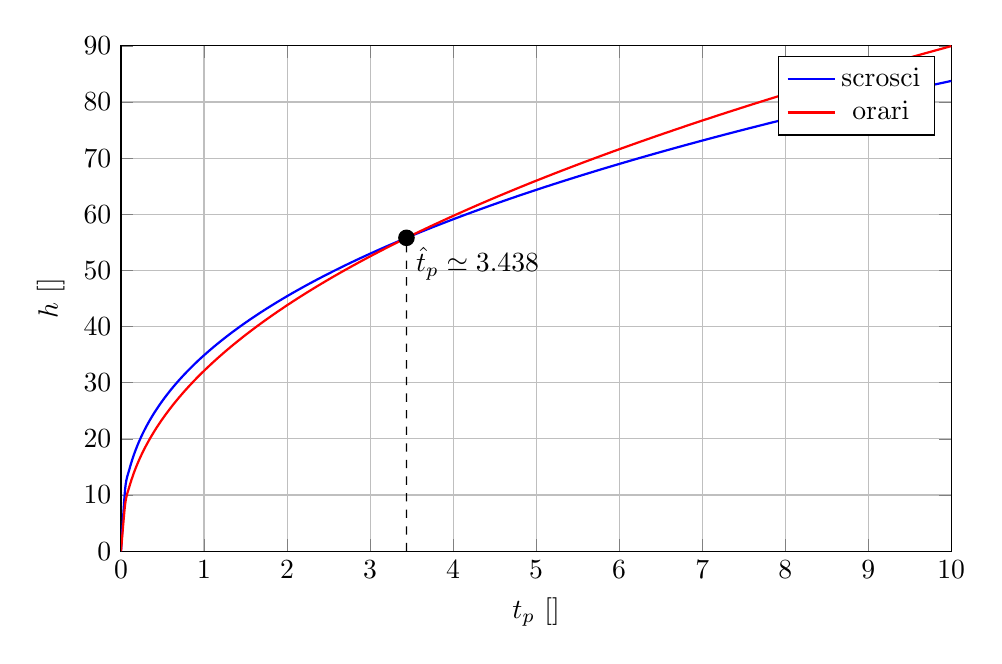
\begin{tikzpicture}
        \begin{axis}[
            xmin = 0, xmax = 10,
            ymin = 0, ymax = 90,
            xtick distance = 1,
            ytick distance = 10,
            height=8cm,
            width=\textwidth,
            grid=major,
            xlabel=$t_p$ \si{[\hour]},
            ylabel=$h$  \si{[\milli\metre]},
            %xtick = {0,0.5,1,1.5,2,2.5,3,3.5,4},
            %title= ,
            /pgf/number format/.cd,
            use comma,
            1000 sep={\,}
        ]
        \addplot [
            domain = 0:10,
            samples = 200,
            smooth,
            thick,
            blue,
        ]{34.890380507986976*x^0.38026437949595393};
        \addplot [
            domain = 0:10,
            samples = 200,
            smooth,
            thick,
            red,
        ]{32.123336325360924*x^0.4471735010272544};
        \legend{scrosci, orari};
        
        \draw[black,dashed] (3.438155,0) -- (3.4381,55.80218)
        node[anchor=north west] {$\hat{t}_p \simeq \SI{3.438}{\hour}$};
        \fill[] (3.4381,55.80218) circle (3pt);
        \end{axis}
    \end{tikzpicture}
    \caption{Curve di possibilità pluviometrica con i parametri $a$ ed $n$ ricavati dalla regressione logaritmica e sostituiti nell'equazione \ref{eq:CPP} con $T_r$ di 25 anni}
    \label{fig:CPPFinale}
\end{figure}